\documentclass{beamer}

\usetheme{metropolis}

\usepackage[style=numeric,sorting=ynt]{biblatex}
\usepackage{minted}
\usepackage[localise]{xepersian}

\settextfont[
  Path = fonts/,
  UprightFont = *-Regular,
  BoldFont = *-Bold,
  ItalicFont = *-Variable
]{Vazir}

\setlatintextfont[
  Path = fonts/,
  UprightFont = *-Regular,
  BoldFont = *-Bold,
  ItalicFont = *-Italic
]{Neuton}

\definecolor{نارنجی}{rgb}{1.0, 0.31, 0.0}

% To force beamer use numbering in captions
\setbeamertemplate{caption}[numbered]{}% Number float-like environments

\setbeamertemplate{footline}[frame number]
\setbeamertemplate{section in toc}[circle]
\setbeamercolor{block body}{bg=lightgray}
\setbeamercolor{headline}{bg=orange}
\setbeamersize{text margin left=1cm,text margin right=1cm}

\setbeamertemplate{headline}
{%
  \begin{beamercolorbox}{section in head/foot}
    \vspace{2pt}\insertnavigation{\paperwidth}\vspace{2pt}
  \end{beamercolorbox}
}

% ---------------------------------------------------------------------------------
% To force beamer use numbering in captions
\setbeamertemplate{caption}[numbered]{}% Number float-like environments

\setbeamertemplate{footline}
{%
  \leavevmode%
  \hbox{%
    \begin{beamercolorbox}[wd=.333333\paperwidth,ht=2.25ex,dp=1ex,center]{author in head/foot}%
      \usebeamerfont{author in head/foot}\insertshortauthor%
    \end{beamercolorbox}%
    \begin{beamercolorbox}[wd=.333333\paperwidth,ht=2.25ex,dp=1ex,center]{title in head/foot}%
      \usebeamerfont{title in head/foot}\insertshorttitle%
    \end{beamercolorbox}%
    \begin{beamercolorbox}[wd=.333333\paperwidth,ht=2.25ex,dp=1ex,right]{date in head/foot}%
      \usebeamerfont{date in head/foot}\hspace*{2em}
      \insertframenumber{} از \inserttotalframenumber{} \hspace*{2ex}%
    \end{beamercolorbox}
  }%
}
\setbeamertemplate{section in toc}[circle]
\setbeamertemplate{blocks}[rounded][shadow=false]
\setbeamercolor{block title}{bg=orange}
\setbeamercolor{block body}{bg=lightgray}
\setbeamersize{text margin left=1cm,text margin right=1cm}
\setbeamertemplate{frametitle continuation}{\insertcontinuationcount}

\AtBeginSection[]
{%
  \begin{frame}
    \frametitle{فهرست}
    \tableofcontents[currentsection]
  \end{frame}
}

\addbibresource{main.bib}

\نویسنده[الهه داستان]{%
  الهه داستان ---
  ۹۶۳۱۰۲۵
  \\
}
\عنوان{پیش‌بینی سرعت ترافیک به وسیله شبکه‌های عصبی}
\subtitle{%
  پروژه کارشناسی\\
  دکتر صفابخش
}
\institute[]{دانشگاه صنعتی امیرکبیر}
\titlegraphic{\vspace{4.5cm}\flushleft
\includegraphics[height=50pt]{img/logo}}
\تاریخ{زمستان ۱۴۰۰}

\begin{document}

\begin{frame}
  \titlepage{}
\end{frame}

\begin{frame}
  \frametitle{فهرست}
  \tableofcontents{}
\end{frame}

\section{مقدمه}

\begin{frame}
  \frametitle{هدف نهایی}
  \begin{block}{}
    مسافرت از یک نقطه مبدا تا یک نقطه مقصد چقدر طول می‌کشد؟
  \end{block}
\end{frame}

\begin{frame}
  \frametitle{هدف}
  \begin{columns}
    \column{.5\textwidth}
    \begin{block}{تعریف}
      پیش‌بینی سرعت ترافیک در یک نقطه جغرافیایی مشخص در یک زمان مشخص
    \end{block}
    \pause
    \begin{block}{مثال}
      فرض کنید که قصد دارید به دانشگاه بروید و می‌خواهید سرعت ترافیک در تئاتر شهر ساعت ۸ صبح را بدانید.
    \end{block}
    \pause
    \column{.45\textwidth}
    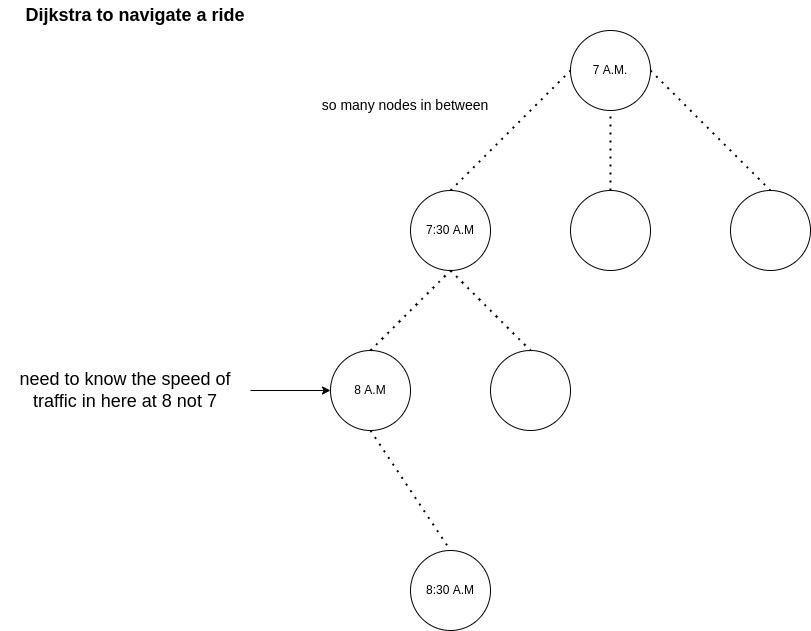
\includegraphics[height=0.5\textheight]{./img/dijkstra.png}
  \end{columns}
\end{frame}

\begin{frame}
  \frametitle{چه کسانی به آن احتیاج دارند؟}
  \begin{columns}
    \column{.25\textwidth}
    
\includegraphics[height=0.5\textheight]{./img/google-maps.png}
    \textbf{Google Maps}\\
    \textit{Google}
    \column{.25\textwidth}
    
\includegraphics[height=0.5\textheight]{./img/waze.png}
    \textbf{Waze}\\
    \textit{Google}
    \column{.25\textwidth}
    
\includegraphics[height=0.5\textheight]{./img/balad.png}
    \textbf{Balad}\\
    \textit{نقشه پردازان ارتباطات نوین}
    \column{.25\textwidth}
    
\includegraphics[height=0.5\textheight]{./img/neshan.png}
    \textbf{Neshan}\\
    \textit{پلتفرم نقشه نشان}
  \end{columns}
\end{frame}

\begin{frame}
  \frametitle{چالش‌ها\cite{2004.08555}}
  \شروع{فقرات}
  \فقره فاکتورهای خارجی
  \فقره داده ترافیکی به صورت زمانی-مکانی
  \شروع{فقرات}
  \فقره وابستگی‌های زمانی پیچیده
  \فقره وابستگی‌های مکانی پیچیده
  \شروع{فقرات}
  \فقره با نزدیک شدن گره‌ها به یکدیگر ارتباط میان آن‌ها بیشتر می‌شود
  \پایان{فقرات}
  \پایان{فقرات}
  \پایان{فقرات}
  \centering
  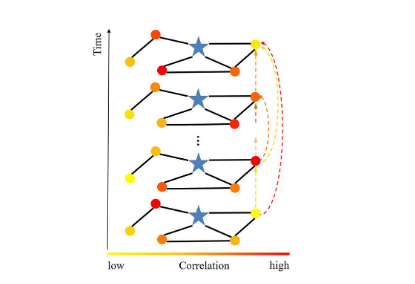
\includegraphics[height=0.5\textheight]{./img/correlations.png}
\end{frame}

\begin{frame}
  \frametitle{تعریف مساله}
  \begin{equation}
    \label{eq:base}
    \hat{v}_{t+1}, \ldots,  \hat{v}_{t+H} = \mathop{\mathrm{argmax}} \log \mathsf{P}({v}_{t+1}, \ldots,  v_{t+H} | v_{t-M+1} , \ldots,  v_{t})
  \end{equation}
  \centering
  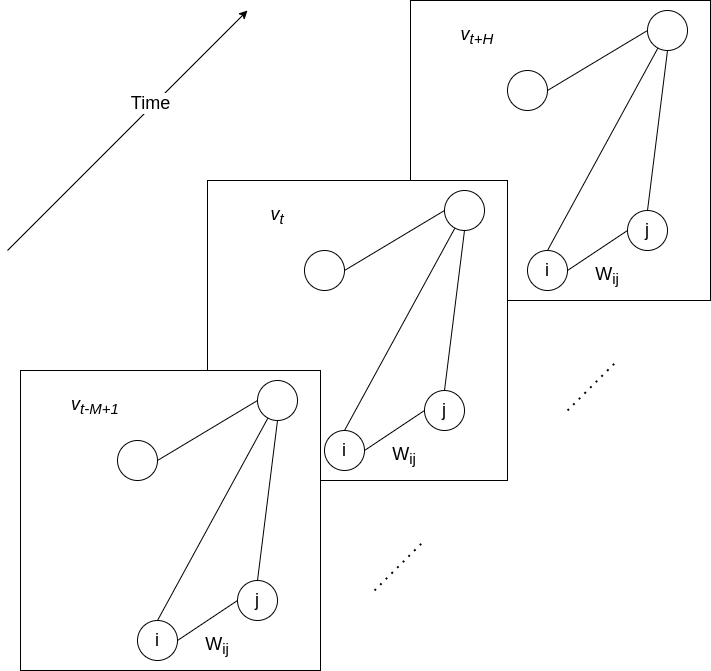
\includegraphics[height=.5\textheight]{img/V.png}
\end{frame}

\section{کارهای مرتبط}

\begin{frame}
  \frametitle{مقدمه\cite{1709.04875}}
  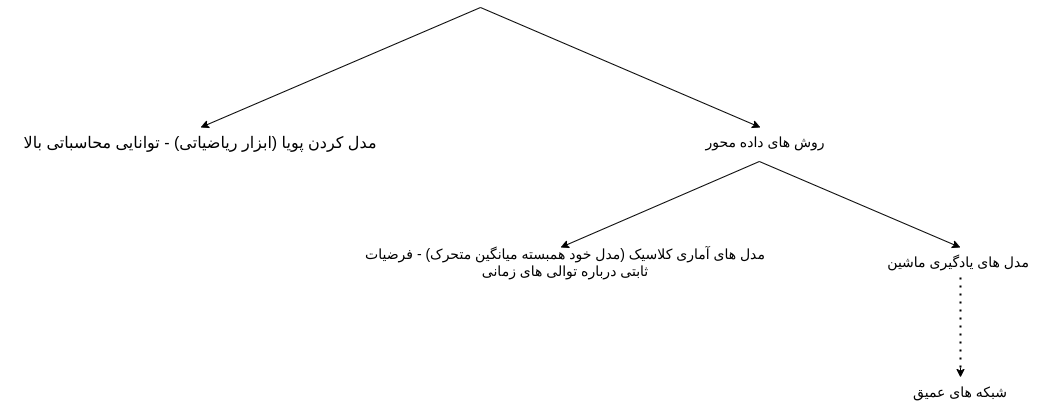
\includegraphics[width=\textwidth]{./img/past.png}
\end{frame}

\begin{frame}
  \frametitle{کارهای مرتبط}
  \شروع{فقرات}
  \فقره \متن‌سیاه{شبکه باور عمیق و کد کننده خودکار پشته‌ای}: برای این شبکه‌های متراکم
  سخت است که ویژگی‌های زمانی و مکانی را به صورت مشترک از ورودی استخراج کنند.
  \فقره \متن‌سیاه{حافظه کوتاه مدت ماندگار}: سنگین از نظر محاسباتی
  \پایان{فقرات}
\end{frame}

\section{راه‌حل پیشنهادی}

\begin{frame}
  \شروع{فقرات}
  \فقره استفاده از هر دو نوع ویژگی زمانی و مکانی
  \فقره در نظر گرفتن مسیرها به صورت گرافی
  \فقره اعمال پیچش به صورت مستقیم بر روی گراف در دامنه طیفی
  \فقره اعمال پیچش بر روی محور زمان
  \پایان{فقرات}
\end{frame}

\begin{frame}
  \frametitle{ورودی راه حل}
  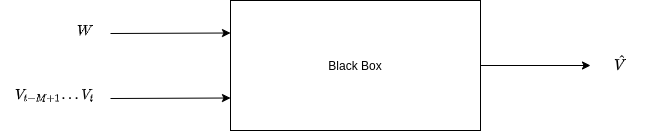
\includegraphics[width=\textwidth]{img/blackbox.png}
\end{frame}

\begin{frame}
  \frametitle{اطلاعات زمانی}
  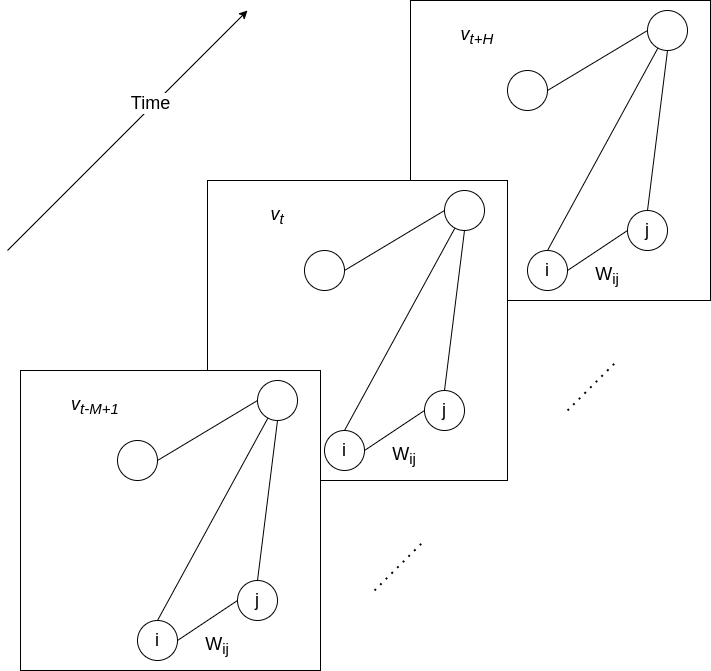
\includegraphics[height=.5\textheight]{img/V.png}
\end{frame}

\begin{frame}
  \frametitle{اطلاعات مکانی}
  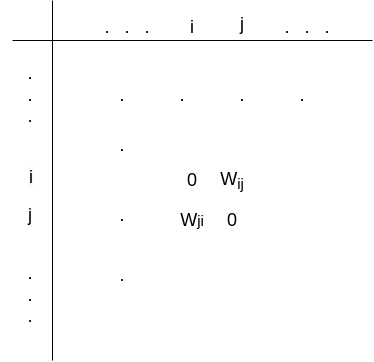
\includegraphics[height=.5\textheight]{img/matrix.png}
  \begin{equation}
    W_{i,j} = \left\{
      \begin{array}{ll}
        \exp(-\frac{d^{2}_{ij}}{\sigma^{2}}) & , i \neq j \quad and \quad \exp(-\frac{d^{2}_{ij}}{\sigma^{2}}) \geq \epsilon \\
        0 & , otherwise. \\
      \end{array}\right.
    \label{eq:distance}
  \end{equation}
\end{frame}

\begin{frame}
  \frametitle{معماری}
  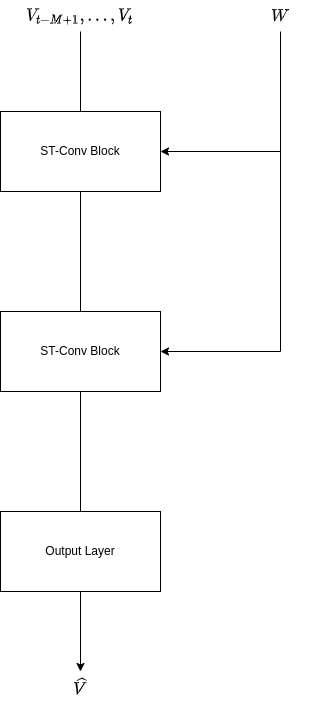
\includegraphics[height=.8\textheight]{img/arch-1.png}
\end{frame}

\begin{frame}
  \frametitle{معماری}
  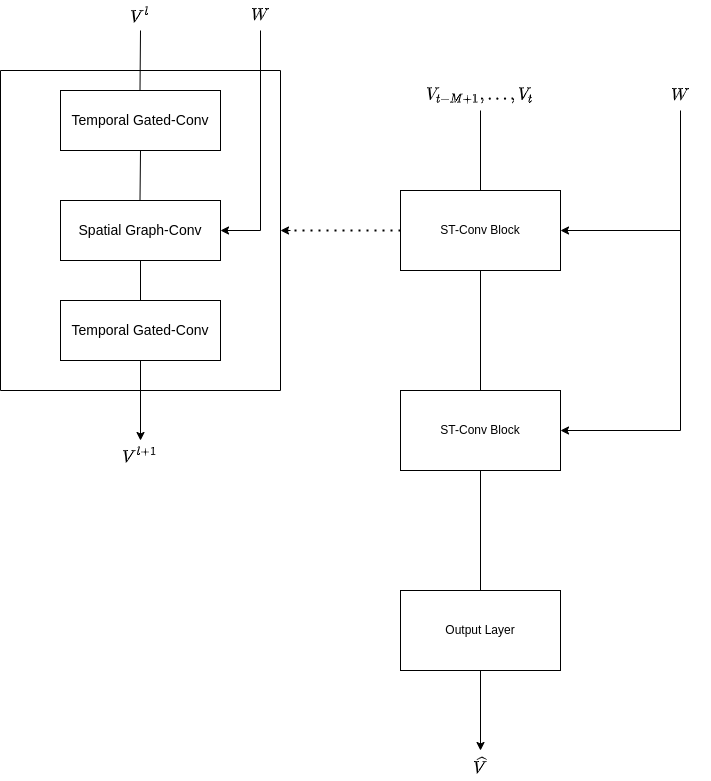
\includegraphics[height=.8\textheight]{img/arch-2.png}
\end{frame}

\begin{frame}
  \frametitle{معماری}
  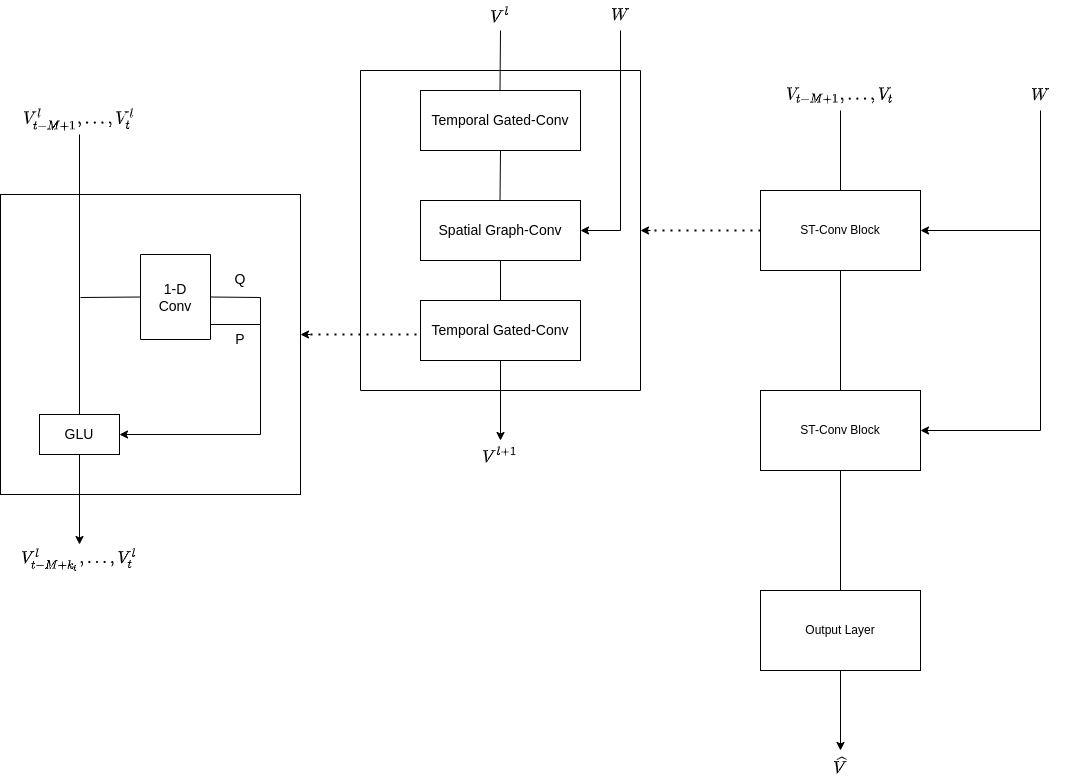
\includegraphics[height=.8\textheight]{img/arch.png}
\end{frame}

\begin{frame}
  \frametitle{پیچش در دامنه طیفی}
  \begin{equation}
    \Theta *_{g} \chi = \Theta(L)\chi = \Theta(U \Lambda U^{T})\chi = U\Theta(\Lambda)U^{T}\chi
    \label{eq:convolution}
  \end{equation}
  \شروع{فقرات}
    \فقره پیچیدگی محاسباتی: $O(n^{2})$
    \فقره چند جمله‌ای چبیشف
    \شروع{فقرات}
      \فقره کاهش پیچیدگی
      \فقره محلی‌سازی
    \پایان{فقرات}
  \پایان{فقرات}
\end{frame}

\begin{frame}
  \frametitle{لایه‌ی پیچشی زمانی}
  \begin{equation}
    \Gamma *_{\tau} Y = P \odot \sigma (Q) \in R^{M-K_{t}+1 \times C_{O}}
    \label{eq:time-conv}
  \end{equation}
\end{frame}

\begin{frame}
  \frametitle{پیش‌بینی چند گام زمانی آینده}
  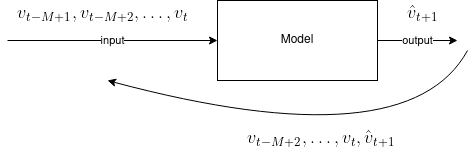
\includegraphics[width=\textwidth]{./img/recursive.png}
\end{frame}

\section{مجموعه‌ی داده‌ها و ارزیابی}

\begin{frame}
  \frametitle{مجموعه دادگان \متن‌لاتین{PeMSD7}}
  \شروع{فقرات}
  \فقره ۲۲۸ ایستگاه اداره حمل و نقل ایالت کالیفرنیا
  \فقره ۱۲ هزار سطر
  \فقره گام زمانی ۵ دقیقه
  \فقره ماه‌های جون و می ۲۰۱۲
  \فقره برگرفته از سنسورها
  \پایان{فقرات}
\end{frame}

\begin{frame}
  \frametitle{مجموعه دادگان اسنپ!}
  \شروع{فقرات}
  \فقره برگرفته از سامانه موقیعت‌یاب جهانی رانندگان
  \پایان{فقرات}
\end{frame}

\begin{frame}
  \frametitle{اطلاعات زمانی}
  \شروع{شمارش}
  \فقره گرفتن دادگان سیستم موقعیت‌یاب جهانی از \متن‌لاتین{NATS}
  \شروع{فقرات}
  \فقره حذف سیگنال‌های کم دقت
  \پایان{فقرات}
  \پایان{شمارش}
  \درج‌تصویر[width=0.8\textwidth]{./img/cron.png}
\end{frame}

\begin{frame}
  \frametitle{اطلاعات زمانی}
  \شروع{شمارش}
  \setcounter{enumi}{1}
  \فقره نگاشت نقطه بر نقشه
  \پایان{شمارش}
  \درج‌تصویر[width=0.5\textwidth]{./img/hmm.png}
  \hfill
  \درج‌تصویر[width=0.3\textwidth]{./img/mapMatch.png}
\end{frame}

\begin{frame}
  \frametitle{اطلاعات زمانی}
  \شروع{شمارش}
  \setcounter{enumi}{2}
  \فقره محاسبه سرعت برای هر راننده
  \پایان{شمارش}
  \درج‌تصویر[width=0.5\textwidth]{./img/speed_per_driver.drawio.png}
  \hfill
  \درج‌تصویر[width=0.3\textwidth]{./img/big-circle-distance.png}
\end{frame}

\begin{frame}
  \frametitle{اطلاعات زمانی}
  \شروع{شمارش}
  \setcounter{enumi}{3}
  \فقره محاسبه سرعت کلی خیابان
  \شروع{فقرات}
  \فقره حذف داده‌های پرت با استفاده از \متن‌لاتین{DBSCAN}
  \پایان{فقرات}
  \پایان{شمارش}
  \درج‌تصویر[width=0.5\textwidth]{./img/bd16594f27b21e22dd897124d5f1a5b5.png}
  \hfill
  \درج‌تصویر[width=0.4\textwidth]{./img/valiasr.png}
\end{frame}

\begin{frame}[fragile]
  \frametitle{اطلاعات مکانی}
  \scriptsize
  \begin{latin}
    \begin{minted}{output}
GET:
    https://api.neshan.org/v1/distance-matrix
      ?origins=36.3177579,59.5323219|36.337115,59.530621
      &destinations=36.35067,59.5451965|36.337005,59.530021
Headers:
Api-Key: YOUR_API_KEY
    \end{minted}
  \end{latin}
\end{frame}

\begin{frame}
  \frametitle{ارزیابی}
  
\includegraphics[height=.5\textheight]{./img/bernard.png}
  \begin{block}{}
  کد در چهارچوب \متن‌لاتین{PyTorch} نوشته شده است.
  \end{block}
\end{frame}

\begin{frame}
  \frametitle{ارزیابی}
  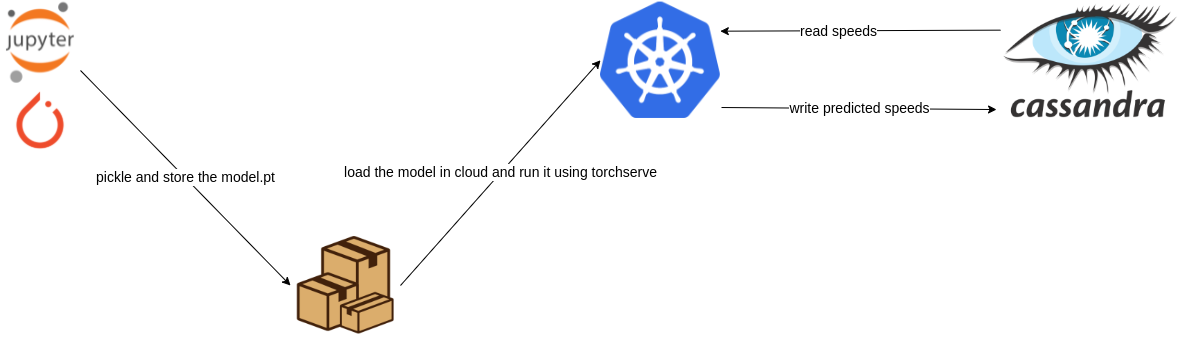
\includegraphics[width=\textwidth]{./img/software.png}
\end{frame}

\begin{frame}
  \frametitle{ارزیابی}
  \شروع{فقرات}
  \فقره مدل ذخیره شده است.
  \فقره مدل روی ابر برده شده است.
  \فقره با استفاده از دستور \متن‌لاتین{torchserve} بالا آمده است.
  \فقره سرعت‌ها از روی \متن‌لاتین{Cassandra} خوانده شده و نتایج پیش‌بینی دوباره داخل \متن‌لاتین{Cassandra} نوشته می‌شوند.
  \پایان{فقرات}
\end{frame}

\begin{frame}
  \frametitle{نتایج ارزیابی}
  \begin{table}[h]
    \centering
    \caption{نتایج اجرا بر روی مجموعه داده‌ی \متن‌لاتین{PeMSD7}}
    \begin{latin}\begin{tabular}{|c|c|c|c|}
      \hline
      Model & MAE (15/30/45 min) & RMSE (15/30/45 min) \\
      \hline
      ARIMA & 5.55/5.86/6.27 & 9.00/9.13/9.38 \\
      \hline
      FNN & 2.74/4.02/5.04 & 4.75/6.98/8.58 \\
      \hline
      FC-LSTM & 3.57/3.94/4.16 & 6.20/7.03/7.51 \\
      \hline
      GCGRU & 2.37/3.31/4.01 & 4.21/5.96/7.13 \\
      \hline
      STGCN(Cheb) & 2.41/3.49/3.81 & 4.27/5.93/7.03 \\
      \hline
    \end{tabular}\end{latin}
  \end{table}
\end{frame}

\begin{frame}
  \frametitle{نتایج ارزیابی}
  \begin{table}[h]
    \centering
    \caption{نتایج اجرا بر روی مجموعه داده‌ی اسنپ!}
    \begin{latin}\begin{tabular}{|c|c|c|c|}
      \hline
      Model & MAE (15/30/45 min) & RMSE (15/30/45 min) \\
      \hline
      STGCN(Cheb) & 3.03/3.98/4.13 & 4.33/6.32/7.89 \\
      \hline
    \end{tabular}\end{latin}
  \end{table}
\end{frame}

\begin{frame}[fragile]
  \frametitle{ارزیابی}
  
\includegraphics[height=.5\textheight]{./img/bernard.png}
  \scriptsize
  \begin{latin}
    \begin{minted}{sql}
SELECT * FROM predictions_by_time_15min_staging
WHERE time_bucket=1828510 AND ref='bd16594f27b21e22dd897124d5f1a5b5'
AND ref_bucket=61;

SELECT * FROM speeds_by_time_15min_staging
WHERE time_bucket=1828512 AND ref='bd16594f27b21e22dd897124d5f1a5b5'
AND ref_bucket=61;
    \end{minted}
  \end{latin}
\end{frame}

\begin{frame}
  \frametitle{نتایج ارزیابی}
  پیش‌بینی سرعت ترافیک برای ۱۵ دقیقه آینده در برابر سرعت‌های واقعی
  \درج‌تصویر[height=.8\textheight]{./img/p1.png}
\end{frame}

\begin{frame}
  \frametitle{نتایج ارزیابی}
  پیش‌بینی سرعت ترافیک برای ۳۰ دقیقه آینده در برابر سرعت‌های واقعی
  \درج‌تصویر[height=.8\textheight]{./img/p2.png}
\end{frame}

\begin{frame}
  \frametitle{نتایج ارزیابی}
  پیش‌بینی سرعت ترافیک برای ۴۵ دقیقه آینده در برابر سرعت‌های واقعی
  \درج‌تصویر[height=.8\textheight]{./img/p3.png}
\end{frame}

\begin{frame}
  \frametitle{نتایج ارزیابی}
  پیش‌بینی سرعت ترافیک برای ۶۰ دقیقه آینده در برابر سرعت‌های واقعی
  \درج‌تصویر[height=.8\textheight]{./img/p4.png}
\end{frame}

\begin{frame}[allowframebreaks]
  \frametitle{مراجع}
  \nocite{*}
  \begin{latin}
  \printbibliography[title=مراجع]
  \end{latin}
\end{frame}

\end{document}
